\documentclass[a4paper,11pt,dvipdfmx]{ujarticle}
% パッケージ
\usepackage{graphicx}
\usepackage{url}
% レイアウト指定を記述したファイルの読み込み
\input{layout}

% タイトルと氏名を変更せよ.
\title{日本におけるデジタル化の状況}
\author{王帅 臻 }

\begin{document}

\maketitle

\section{デジタル競争力ランキング}

国際経営開発研究所(IMD)の調査\cite{imd}によると、日本のデジタル競争力のランキングは図\ref{fig:imd_ranking}に示すように、調査対象の64カ国中、総合で28位、知識分野で25位となっている。

\begin{figure}[htbp]
\centering
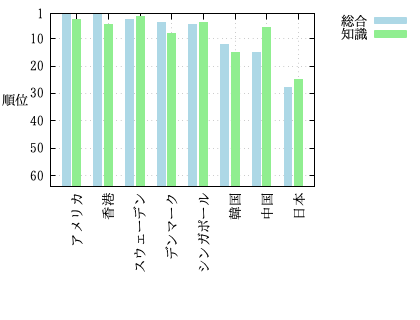
\includegraphics[width=0.88\linewidth]{fig31.png}
\caption{デジタル競争力ランキング(64カ国中)}
\label{fig:imd_ranking}
\end{figure}
\newpage
\section{ブロードバンドの整備状況}

OECDによるブロードバンド回線の普及に関する調査\cite{oecd}によると、表\ref{tbl:競争力ランキング}に示すように、日本における 100人あたりのモバイルブロードバンドの加入者数は190.5で、第1位になっている。2位はエストニア
で、3位米国と続く。

\begin{table}[htbp]
    \centering
    \caption{モバイルブロードバンドの加入者数(100人あたり)}\label{tbl:競争力ランキング}

    \begin{tabular}{|c|l|r|}
        \hline
        順位 & 国名 & 加入者数 \\
        \hline
        1位 & 日本 & 190.5 \\
        \hline
        2位 & エストニア & 179.9 \\
        \hline
        3位 & 米国 & 169.0 \\
        \hline
        4位 & フィンランド & 157.0 \\
        \hline
        5位 & デンマーク & 141.7 \\
        \hline
        6位 & ラトビア & 141.6 \\
        \hline
        7位 & イスラエル & 139.9 \\
        \hline
        8位& オランダ & 133.7 \\
        \hline
        9位 & ポーランド & 131.3 \\
        \hline
        10位 & スウェーデン & 127.2 \\
        \hline
    \end{tabular}
\end{table}

\section{考察}

\begin{itemize}
  \item 日本のデジタル競争力世界ランキングで低い位置にある。そのため世界から見たら日本は最先端であるとは言えずまだまだ課題があると感じる。
  \item 日本のブロードバンド回線は普及率世界で一番高い。しかしデジタルのランキングでは最下位である。これはまだまだ、日本がデジタルの生活が世界よりも普及してないからではないかと考えられる。
\end{itemize}

\bibliographystyle{junsrt}
\bibliography{exercise.bib}

\end{document}